% arara: lualatexprepend: { options: [ '\providecommand{\videoFrames}{2}', '\providecommand{\tikzFrames}{1}' ] }
% arara: lualatexprepend: { options: [ '\providecommand{\videoFrames}{240}', '\providecommand{\tikzFrames}{60}' ] }

\providecommand{\importPath}{../../../../Shared/Imports}
\providecommand{\assetPath}{../../../../Assets}
\providecommand{\sharedPath}{../../../../Shared}
\providecommand{\plotCodePath}{../../../../Assets}

\documentclass[tikz, crop=false, float=false]{standalone}

\usepackage[mode=buildnew, subpreambles=false]{standalone}
\usepackage{import}
\usepackage{hyperref}
\usepackage[tbtags]{amsmath}
\usepackage{amsfonts}
\usepackage{amssymb}
\usepackage[T1]{fontenc}
\usepackage{siunitx}
\usepackage{chemformula}
\usepackage{catchfilebetweentags}
\usepackage[style=ieee,backend=biber]{biblatex}
\usepackage{csvsimple}
\usepackage{longtable}
\usepackage{float}
\usepackage{graphicx}

\usepackage{tikz}
    \usetikzlibrary{math, arrows, circuits.ee.IEC, positioning, shapes.arrows, shapes.geometric, external}
\usepackage{pgfplots}
    \pgfplotsset{compat=newest, compat/show suggested version=false}
    \usepgfplotslibrary{groupplots}
\usepackage[siunitx,american voltages, american currents, RPvoltages]{circuitikz}
\usepackage{tikzscale}

\usepackage{animate}
\usepackage[debug, toc, section=section, acronym, symbols]{glossaries} % Glossaries package

%Get rounded wire jumps
\tikzset{
    declare function={% in case of CVS which switches the arguments of atan2
        atan3(\a,\b)=ifthenelse(atan2(0,1)==90, atan2(\a,\b), atan2(\b,\a));},
        kinky cross radius/.initial=+.125cm,
        @kinky cross/.initial=+, kinky crosses/.is choice,
        kinky crosses/left/.style={@kinky cross=-},kinky crosses/right/.style={@kinky cross=+},
        kinky cross/.style args={(#1)--(#2)}{
        to path={
          let \p{@kc@}=($(\tikztotarget)-(\tikztostart)$),
              \n{@kc@}={atan3(\p{@kc@})+180} in
          -- ($(intersection of \tikztostart--{\tikztotarget} and #1--#2)!%
                 \pgfkeysvalueof{/tikz/kinky cross radius}!(\tikztostart)$)
          arc [ radius     =\pgfkeysvalueof{/tikz/kinky cross radius},
                start angle=\n{@kc@},
                delta angle=\pgfkeysvalueof{/tikz/@kinky cross}180 ]
          -- (\tikztotarget)}}
      }

% SI unit pkg conf
\sisetup{
    load-configurations = abbreviations,
    detect-family = true,
    per-mode = reciprocal
}%

% Bibliography .bib file locations should maybe be local?
\addbibresource[location=local]{\sharedPath/bibFiles/accelerators.bib}

% Other Configurations

% Alphabetize glossary and acronyms list
\makeglossaries



\begin{document}
    \directlua{
        path = "\plotCodePath"
        lorenz = require(path.."/Code/lorenzAnim")
    }
    \newcommand\addLUADEDplot[5][]{%
        \directlua{
            #5 = lorenz.LorenzAttractor(#2,#3,#4,#5,[[#1]])
        }%
    }
    \begin{animateinline}[poster=last, controls, buttonsize=1.0em]{12}
        \multiframe{\tikzFrames}{iTer=0+1}{
                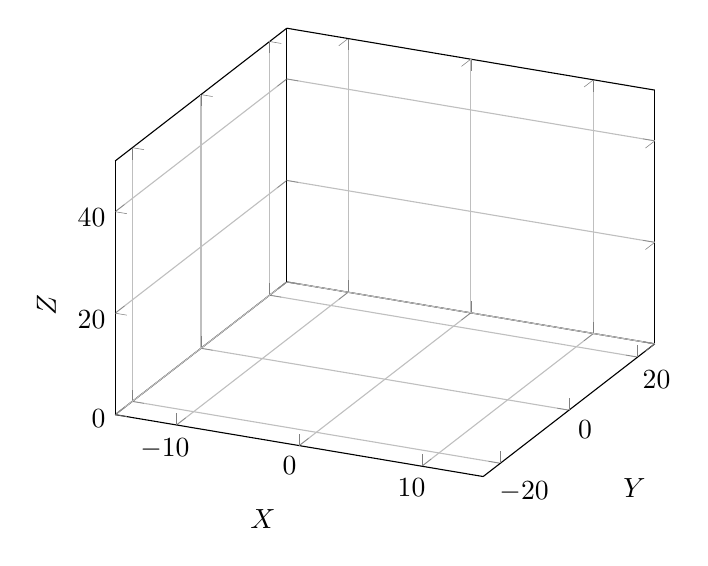
\begin{tikzpicture}
                    \begin{axis}[grid=both,
                        xlabel=$X$,
                        ylabel=$Y$,
                        zlabel=$Z$,
                        xmin=-15,
                        xmax=15,
                        ymin=-25,
                        ymax=25,
                        zmin=0,
                        zmax=50,]
                        \addLUADEDplot[color=red,smooth]{0.02}{10}{\iTer}{red1};
                        \addLUADEDplot[color=green,smooth]{0.02}{10}{\iTer}{green1};
                        \addLUADEDplot[color=blue,smooth]{0.02}{10}{\iTer}{blue1};
                        \addLUADEDplot[color=cyan,smooth]{0.02}{10}{\iTer}{cyan1};
                        \addLUADEDplot[color=magenta,smooth]{0.02}{10}{\iTer}{magenta1};
                        \addLUADEDplot[color=yellow,smooth]{0.02}{10}{\iTer}{yellow1};
                    \end{axis}
                \end{tikzpicture}
            }
    \end{animateinline}
\end{document}
